% Ctrl + alt + b to build & preview (Linux)
\documentclass[11pt,a4paper]{article}

\usepackage[margin=1in, paperwidth=8.3in, paperheight=11.7in]{geometry}
\usepackage{amsfonts}
\usepackage{amsmath}
\usepackage{enumerate}
\usepackage{enumitem}
\usepackage{fancyhdr}
\usepackage{graphicx}
\usepackage{mathtools}
\usepackage{setspace}

\begin{document}

\pagestyle{fancy}
\setlength\parindent{0pt}
\allowdisplaybreaks

\renewcommand{\headrulewidth}{0pt}
\newcommand{\vect}[1]{\boldsymbol{#1}}
\newcommand{\dotprod}[0]{\boldsymbol{\cdot}}
\newcommand{\real}[0]{\mathbb{R}}
\newcommand{\field}[0]{\mathbb{F}}
\newcommand{\complex}[0]{\mathbb{C}}
\newcommand{\innerproduct}[2]{\langle #1, #2 \rangle}

% Cover page title
\title{Linear Algebra \& Geometry - Application Notes}
\author{Dom Hutchinson}
\date{\today}
\maketitle

% Header
\fancyhead[L]{Dom Hutchinson}
\fancyhead[C]{Linear Algebra \& Geometry - Application Notes}
\fancyhead[R]{\today}

\textbf{How to convert a series of linear equations to an augmented matrix.}\\

\underline{\textit{Process}}\\
When given a series of $n$ linear equations, each with the same $m$, then an augmented $(n+1) \times m$ matrix can be formed.
\begin{enumerate}[label=\roman*)]
  \itemsep0em
  \item Set the first $n$ elements of each \textit{row} of the matrix to be the coefficients for one of the linear equations.
  \item Set the \textit{last} element of the row to be the value of this linear equation.
\end{enumerate}

\underline{\textit{Example}}\\
Convert the following linear equations to an augment matrix
$$x + z = 1, 2x - 2y = 1\ \&\ - 3y - 3x = -1$$
\begin{center}$\begin{pmatrix*}[r] 1 & 0 & 1 & 1 \\ 2 & -2 & 0 & 1 \\ 0 & -3 & -3 & -1\end{pmatrix*}$\end{center}

\textbf{How to solve a series of linear equations using an augmented matrix.}\\

\underline{\textit{Theory}}\\
The following elementary row operations can be carried out without altering the solution of an augmented matrix.
\begin{enumerate}[label=\roman*)]
  \itemsep0em
  \item row $i \mapsto \lambda$row $i$ for $\lambda \in \real\backslash \{0\}$;
  \item row $i \mapsto$ row $i + \lambda$ row $j$ for $\lambda \in \real\backslash \{0\}$; and,
  \item row $j \mapsto$ row $i\ \&\ $ row $i \mapsto$ row $j$.
\end{enumerate}

\underline{\textit{Process}}
\begin{enumerate}[label=\roman*)]
  \itemsep0em
  \item Convert the linear equations into an augmented matrix;
  \item Perform elementary rows operations until the \textit{first} $n$ rows and columns form an identity matrix; and,
  \item The values in the \textit{last} column are the solutions.
\end{enumerate}

\newpage\underline{\textit{Example}}\\
Solve the following system of linear equations
$$x+y+2z=9, 2x+4y-3z=1\ \&\ 3x+6y-5z=0$$
\[\begin{array}{ccccc}
  \begin{pmatrix*}[r] 1 & 1 & 2 & 9 \\ 2 & 4 & -3 & 1 \\ 3 & 6 & -5 & 0 \end{pmatrix*} &=& \begin{pmatrix*}[r] 1 & 1 & 2 & 9 \\ 0 & 2 & -7 & -17 \\ 0 & 3 & -11 & -27 \end{pmatrix*} &=& \begin{pmatrix*}[r] 1 & 1 & 2 & 9 \\ 0 & 2 & -7 & -17 \\ 0 & 1 & -4 & -10 \end{pmatrix*}\\
  &=& \begin{pmatrix*}[r] 1 & 1 & 2 & 9 \\ 0 & 0 & 1 & 3 \\ 0 & 1 & -4 & -10 \end{pmatrix*} &=& \begin{pmatrix*}[r] 1 & 1 & 2 & 9 \\ 0 & 1 & -4 & -10 \\ 0 & 0 & 1 & 3 \end{pmatrix*} \\
  &=& \begin{pmatrix*}[r] 1 & 1 & 0 & 3 \\ 0 & 1 & 0 & 2 \\ 0 & 0 & 1 & 3 \end{pmatrix*} &=& \underline{\begin{pmatrix*}[r] 1 & 0 & 0 & 1 \\ 0 & 1 & 0 & 2 \\ 0 & 0 & 1 & 3 \end{pmatrix*}}
\end{array}\]
So the only solution to this system of linear equations is $x=1,y=2\ \&\ z=3$.\\

\textbf{How to find the Determinant}\\

\underline{\textit{Process}}\\
The determinant can be found using \textit{Laplace's Rule}.
$$det(A) = \sum_{j=1}^n a_{ij}.(-1)^{i+j}.det(A_{ij}) \mathrm{\ for\ a\ fixed\ }i$$
Where $A_{ij}$ is the matrix $A$ without its \underline{$i^{th}$ row and $j^{th}$ column.}\\

\underline{\textit{Example}}\\
Find the determinant of $\begin{pmatrix} 1 & 2 & 3 \\ 4 & 5 & 6 \\ 7 & 8 & 9 \end{pmatrix}$.
\setstretch{1.2}
\[\begin{array}{ccl}
  \begin{vmatrix} 1 & 2 & 3 \\ 4 & 5 & 6 \\ 7 & 8 & 9 \end{vmatrix} &=& 1\begin{vmatrix} 5 & 6 \\ 8 & 9 \end{vmatrix} - 2\begin{vmatrix} 4 & 6 \\ 7 & 9 \end{vmatrix} + 3\begin{vmatrix} 4 & 5 \\ 7 & 8 \end{vmatrix}\\
    &=& 1[5 \times 9 - 6 \times 8] - 2[4 \times 9 - 6 \times 7] + 3[4 \times 8 - 5 \times 7] \\
    &=& 1(-3) -2(-6) + 3(-3) \\
    &=& -3 + 12 - 9\\
    &=& \underline{0}
\end{array}\]
\setstretch{1}

\textbf{How to Invert a Matrix}\\

\underline{\textit{Theory}}\\
A matrix is \textit{invertible} iff $det(A) \neq 0$.\\
An inverted matrix, $A^{-1}$, obeys $AA^{-1} = I$.\\
The \textit{adjoint} of a matrix can be found using
$$(adj(A))_{ij} = (-1)^{i+j}det(A^t_{ij})$$
Where $A^t_{ij}$ is the transpose of matrix $A$ without its \underline{$i^{th}$ row and $j^{th}$ column.}\\

\underline{\textit{Process}}\\
The inverse of a matrix $A$ can be found by
$$A^{-1} = \frac{adj(A)}{det(A)}$$

\textit{\underline{\textit{Example of Adjoint Matrix}}}\\
Find the adjoint of $A = \begin{pmatrix} 1 & 2 & 3 \\ 4 & 5 & 6 \\ 7 & 8 & 9 \end{pmatrix}$.
\[\begin{array}{rcl}
  A^t &=& \begin{pmatrix} 1 & 4 & 7 \\ 2 & 5 & 8 \\ 3 & 6 & 9\end{pmatrix}\\
  adj(A) &=& \begin{pmatrix} +\begin{vmatrix} 5 & 8 \\ 6 & 9 \end{vmatrix} & -\begin{vmatrix} 2 & 8 \\ 3 & 9 \end{vmatrix} & +\begin{vmatrix} 2 & 5 \\ 3 & 6 \end{vmatrix} \\ -\begin{vmatrix} 4 & 7 \\ 6 & 9 \end{vmatrix} & + \begin{vmatrix} 1 & 7 \\ 3 & 9\end{vmatrix} & -\begin{vmatrix} 1 & 4 \\ 3 & 6\end{vmatrix} \\ +\begin{vmatrix} 4 & 7 \\ 5 & 8 \end{vmatrix} & -\begin{vmatrix} 1 & 7 \\ 2 & 8 \end{vmatrix} & +\begin{vmatrix} 1 & 4 \\ 2 & 5 \end{vmatrix} \end{pmatrix}\\
  &=& \underline{\begin{pmatrix*}[r] -3 & 6 & -3 \\6 & -12 & 6 \\ -3 & 6 & -3 \end{pmatrix*}}
\end{array}\]

\newpage\textit{\underline{\textit{Example of Inverse Matrix}}}\\
Find the inverse of $A = \begin{pmatrix} 1 & 2 & 3 \\ 0 & 1 & 4 \\ 5 & 6 & 0 \end{pmatrix}$
\[\begin{array}{rcl}\setstretch{1.2}
  A^t &=& \begin{pmatrix} 1 & 0 & 5 \\ 2 & 1 & 6 \\ 3 & 4 & 0 \end{pmatrix}\\
  adj(A) &=& \begin{pmatrix} +\begin{vmatrix} 1 & 6 \\ 4 & 0\end{vmatrix} & -\begin{vmatrix}2 & 6 \\ 3 & 0 \end{vmatrix} & +\begin{vmatrix}2 & 1 \\ 3 & 4 \end{vmatrix} \\ -\begin{vmatrix} 0 & 5 \\ 4 & 0\end{vmatrix} & +\begin{vmatrix}1 & 5 \\ 3 & 0 \end{vmatrix} & -\begin{vmatrix}1 & 0 \\ 3 & 4 \end{vmatrix} \\ +\begin{vmatrix} 0 & 5 \\ 1 & 6\end{vmatrix} & -\begin{vmatrix} 0 & 5 \\ 2 & 6 \end{vmatrix} & +\begin{vmatrix}1 & 0 \\ 2 & 1 \end{vmatrix} \end{pmatrix}\\
  &=& \begin{pmatrix*}[r] -24 & 18 & 5 \\ 20 & -15 & -4 \\ -5 & 4 & -1 \end{pmatrix*}\\
  det(A) &=& 1\begin{vmatrix} 1 & 4 \\ 6 & 0\end{vmatrix} -2\begin{vmatrix}0 & 4 \\ 5 & 0 \end{vmatrix} +3\begin{vmatrix}0&1\\5&6 \end{vmatrix}\\
  &=& -24+40-15\\
  &=& 1\\
  A^{-1} &=& \displaystyle{\frac{adj(A)}{det(A)}}\\
  &=& \displaystyle{\frac{1}{1}\begin{pmatrix*}[r] -24 & 18 & 5 \\ 20 & -15 & -4 \\ -5 & 4 & -1 \end{pmatrix*}}\\
  &=& \underline{\begin{pmatrix*}[r] -24 & 18 & 5 \\ 20 & -15 & -4 \\ -5 & 4 & -1 \end{pmatrix*}}
\setstretch{1}\end{array}\]

\textbf{How to Form a Basis}\\

\underline{\textit{Theory}}\\
Let $V$ be a vector space.\\
Then $\{ v_1, \dots, v_n\}$ are a basis for $V$ if they are all linearly independent\\ and $V = span(\{v_1, \dots, v_n\})$.\\

\underline{\textit{Process}}\\
Let $v_1, \dots , v_n \in V$ and $\{ w_1, \dots , w_n\}$ be a basis, to be formed, for $V$.
\begin{enumerate}[label=\roman*)]
  \itemsep0em
  \item Construct the augmented matrix $\begin{pmatrix} v_1 & \dots & v_n & 0 \end{pmatrix}$;
  \item Reduce this matrix to row echeldon form;
  \item Identify the vectors which are associated to columns with the leading $1$s. These vectors form a basis for the rest.
\end{enumerate}

\newpage\underline{\textit{Example}}\\
Find a basis for $\left\{ \begin{pmatrix} 1 \\ 2 \\ 1 \end{pmatrix}, \begin{pmatrix*}[r] -1 \\ -1 \\ 1 \end{pmatrix*}, \begin{pmatrix} 1 \\ 4 \\ 5 \end{pmatrix}, \begin{pmatrix*}[r] 3 \\ 4 \\ -1\end{pmatrix*}, \begin{pmatrix} 0 \\ 1 \\ 2 \end{pmatrix}, \begin{pmatrix} 4 \\ 9 \\ 6 \end{pmatrix}  \right\}$.
\[\begin{array}{rcl}
\mathrm{Augmented\ matrix} & & \begin{pmatrix*}[r] 1 & -1 & 1 & 3 & 0 & 4 & 0 \\ 2 & -1 & 4 & 4 & 1 & 9 & 0 \\ 1 & 1 & 5 & -1 & 2 & 6 & 0  \end{pmatrix*}\\
&=& \begin{pmatrix*}[r] 1 & -1 & 1 & 3 & 0 & 4 & 0 \\ 0 & 1 & 2 & -2 & 1 & 1 & 0 \\ 0 & 2 & 4 & -4 & 2 & 2 & 0 \end{pmatrix*}\\
&=& \begin{pmatrix*}[r] 1 & -1 & 1 & 3 & 0 & 4 & 0 \\ 0 & 1 & 2 & -2 & 1 & 1 & 0 \\ 0 & 0 & 0 & 0 & 0 & 0 & 0 \end{pmatrix*}
\end{array}\]
So the first \& second vectors, $\begin{pmatrix} 1 \\ 2 \\ 1 \end{pmatrix}\ \&\ \begin{pmatrix*}[r] -1 \\ -1 \\ 1 \end{pmatrix*}$, form a basis for the rest of the vectors.\\

\textbf{How to Check is a Basis is Orthogonal}\\

\underline{\textit{Theory}}\\
Let $V$ be a vector space and $v, w \in V$.\\
Then $v\ \&\ w$ are orthogonal if
$$v \dotprod w = 0$$
This means $v\ \&\ w$ are at $\frac{\pi}{2}rads$ to each other.\\
A basis, $\{v_1, \dots, v_n\}$ , is orthogonal if
$$v_i \dotprod v_j = 0\mathrm{\ iff\ } i \neq j$$

\underline{\textit{Process}}\\
Say we are given $n$ vectors.\\
Then we need to check the \textit{dot product} of all possible combinations obey the conditions.\\
As $v \dotprod w = w \dotprod v\ \forall\ v, w$ then there are $\frac{1}{2}n(n+1)$ such combinations.\\

\underline{\textit{Example}}\\
Are $\vect{v}_1 = \begin{pmatrix*}[r] -1 \\ 2 \\1 \end{pmatrix*}, \vect{v}_2 = \begin{pmatrix} 1 \\ 0 \\ 1 \end{pmatrix}\ \&\ \vect{v}_3 = \begin{pmatrix*}[r] -1 \\ -1 \\ 1\end{pmatrix*}$ orthogonal.
\[\begin{array}{rclcl}
  \vect{v}_1 \dotprod \vect{v}_1 &=& 1 + 4 + 1 &=& 6\\
  \vect{v}_1 \dotprod \vect{v}_2 &=& -1 + 0 + 1 &=& 0\\
  \vect{v}_1 \dotprod \vect{v}_3 &=& 1 -2 + 1 &=& 0\\
  \vect{v}_2 \dotprod \vect{v}_2 &=& 1 + 0 + 1 &=& 2\\
  \vect{v}_2 \dotprod \vect{v}_3 &=& -1 + 0 + 1 &=& 0\\
  \vect{v}_3 \dotprod \vect{v}_3 &=& 1 + 1 + 1 &=& 3
\end{array}\]
Yes they are.\\

\newpage\textbf{How to Prove a Map is a Linear Map}\\

\underline{\textit{Theory}}\\
A map, $T$, is a linear map if
\begin{enumerate}[label=\roman*)]
  \itemsep0em
  \item $T(x + y) = T(x) + T(y)\ \forall\ x, y$; and,
  \item $T(\lambda x) = \lambda T(x)$.
\end{enumerate}

\underline{\textit{Process}}\\
Need to prove both of these are conditions are true in all cases.\\

\underline{\textit{Example}}\\
Prove that $T : \real^2 \to \real^3$ defined as $T\begin{pmatrix} x \\ y \end{pmatrix} = \begin{pmatrix} x \\ y \\ x+2y \end{pmatrix}$ is a linear map.\\
Let $\vect{x} = \begin{pmatrix} x_1 \\ x_2 \end{pmatrix},\ \vect{y} = \begin{pmatrix} y_1 \\ y_2 \end{pmatrix}$ and $\lambda \in \real$.
\[\begin{array}{rcl}
  T(\vect{x} + \vect{y}) &=& T\left(\begin{pmatrix} x_1 \\ x_2 \end{pmatrix} + \begin{pmatrix} y_1 \\ y_2 \end{pmatrix} \right)\\
  &=& T\left( \begin{pmatrix} x_1 + x_1 \\ x_2 + y_2 \end{pmatrix} \right)\\
  &=& \begin{pmatrix} x_1 + y_1 \\ x_2 + y_2 \\ x_1 + y_1 + 2x_2 + 2y_2 \end{pmatrix}\\
  &=& \begin{pmatrix} x_1 + y_1 \\ x_2 + y_2 \\ (x_1 + 2x_2) + (y_1 + 2y_2) \end{pmatrix}\\
  &=& \begin{pmatrix} x_1 \\ x_2 \\ x_1 + 2x_2 \end{pmatrix} + \begin{pmatrix} y_1 \\ y_2 \\ y_1 + 2y_2 \end{pmatrix}\\
  &=& T(\vect{x}) + T(\vect{y})\\\\
  T(\lambda\vect{x}) &=& T\left( \begin{pmatrix} \lambda x_1 \\ \lambda x_2 \end{pmatrix}\right)\\
  &=& \begin{pmatrix} \lambda x_1 \\ \lambda x_2 \\ \lambda x_1 + 2\lambda x_2 \end{pmatrix}\\
  &=& \begin{pmatrix} \lambda x_1 \\ \lambda x_2 \\ \lambda (x_1 + 2x_2) \end{pmatrix}\\
  &=& \lambda\begin{pmatrix} x_1 \\ x_2 \\ x_1 + 2x_2 \end{pmatrix}\\
  &=& \lambda T(\vect{x})
\end{array}\]
$T$ is a linear map.\\

\newpage\textbf{How to Represent a Linear Map as a Matrix}\\

\underline{\textit{Process}}\\
Let $T : \real^n \to \real^m$ be a linear map.\\
Then $T$ can be represented by the matrix $M_T \in M_{m, n}(\real)$ where $M_Tx = T(x)$.
$$t_{ij} = e_i \dotprod T(e_j),\quad e_j \in \real^n\ \&\ e_i \in \real^m$$
Perform this for all combinations of $i \in [1, m]\ \&\ j \in [1, n]$\\

\underline{\textit{Example}}\\
Write $T : \real^2 \to \real^3$ defined as $T\begin{pmatrix} x \\ y \end{pmatrix} = \begin{pmatrix} x \\ y \\ x+2y \end{pmatrix}$ as a matrix.
\[T(\vect{e}_1) = \begin{pmatrix} 1 \\ 0 \\ 1 \end{pmatrix}\ \&\ T(\vect{e}_2) = \begin{pmatrix} 0 \\ 1 \\ 2 \end{pmatrix}\]
\[\begin{array}{rcccclcl}
t_{11} &=& \vect{e}_1 \dotprod T(\vect{e}_1) &=& (1, 0, 0) \dotprod (1, 0 ,1) &=& 1 + 0 + 0 = 1\\
t_{12} &=& \vect{e}_2 \dotprod T(\vect{e}_1) &=& (1, 0, 0) \dotprod (0, 1 ,2) &=& 0 + 0 + 0 = 0\\
t_{21} &=& \vect{e}_2 \dotprod T(\vect{e}_1) &=& (0, 1, 0) \dotprod (1, 0 ,1) &=& 0 + 0 + 0 = 0\\
t_{22} &=& \vect{e}_2 \dotprod T(\vect{e}_2) &=& (0, 1, 0) \dotprod (0, 1 ,2) &=& 0 + 1 + 0 = 1\\
t_{31} &=& \vect{e}_3 \dotprod T(\vect{e}_1) &=& (0, 0, 1) \dotprod (1, 0 ,1) &=& 0 + 0 + 1 = 1\\
t_{32} &=& \vect{e}_3 \dotprod T(\vect{e}_2) &=& (0, 0, 1) \dotprod (0, 1 ,2) &=& 0 + 0 + 2 = 2\\
M_T &=& \underline{\begin{pmatrix} 1 & 0 \\ 0 & 1 \\ 1 & 2\end{pmatrix}}
\end{array}\]

\textbf{How to Find the Cross Product}\\

\underline{\textit{Theory}}\\
The cross product is a vector which is perpendicular to the plane formed by two other vectors in $\real^3$.\\
The magnitude of this vector is equal to the area parallelogram formed with these two vectors as the sides.\\
The cross product is denoted as $\vect{x} \times \vect{y}$.\\

\underline{\textit{Process}}\\
$\vect{x} \times \vect{y} = \begin{vmatrix} \vect{e}_1 & \vect{e}_2 & \vect{e}_3 \\ x_1 & x_2 & x_3 \\ y_1 & y_2 & y_3 \end{vmatrix} = \vect{e}_1\begin{vmatrix} x_2 & x_3 \\ y_2 & y_3 \end{vmatrix} - \vect{e}_2\begin{vmatrix} x_1 & x_3 \\ y_1 & y_3 \end{vmatrix} + \vect{e}_3\begin{vmatrix} x_1 & x_2 \\ y_1 & y_2 \end{vmatrix}$\\

\newpage\underline{\textit{Example}}\\
Let $\vect{v} = \begin{pmatrix*}[r] 3 \\ -1 \\ 5 \end{pmatrix*}$ and $\vect{w} = \begin{pmatrix*}[r] 0 \\ 4 \\ -2 \end{pmatrix*}$. Compute $\vect{v} \times \vect{w}$.
\[\begin{array}{rcl}
  \vect{v} \times \vect{w} &=& \begin{vmatrix*}[r] \vect{e}_1 & \vect{e}_2 & \vect{e}_3 \\ 3 & -1 & 5 \\ 0 & 4 & -2\end{vmatrix*}\\
  &=& \vect{e}_1 \begin{vmatrix*}[r] -1 & 5 \\ 4 & -2 \end{vmatrix*} - \vect{e}_2 \begin{vmatrix*}[r] 3 & 5 \\ 0 & -2 \end{vmatrix*} + \vect{e}_3 \begin{vmatrix*}[r] 3 & -1 \\ 0 & 4 \end{vmatrix*}\\
  &=& \vect{e}_1(-18) - \vect{e}_2(-6) + \vect{e}_3(12)\\
  &=& \underline{\begin{pmatrix*}[r] -18 \\ 6 \\ 12 \end{pmatrix*}}
\end{array}\]

\textbf{How to prove a Set is a Vector Space}\\

\underline{\textit{Theory}}\\
A \textit{field} is a set of numbers for which addition \& multiplication are defined.\\
A \textit{vector space} is aset of vectors which are part of a field and obey the following conditions.
\begin{enumerate}[label=\roman*)]
  \itemsep0em
  \item $V$ is abelian wrt addition, $v + w = w + v\ \forall\ v, w \in V$;
  \item $\lambda v \in V\ \forall\ \lambda \in \field, v \in V$;
  \item $\lambda(v + w) = \lambda v + \lambda w$;
  \item $\lambda(\mu v) = (\lambda\mu)v$; and,
  \item $1.v = v$.
\end{enumerate}

\underline{\textit{Process}}\\
Need to prove these are conditions are true in all cases.\\

\underline{\textit{Example}}\\
Let $V \subset \real^2$ be defined by $V = \{(v, 2v) : v \in \real \}$\\
Show $V$ is a vector space over $\real$.\\

Let $\vect{x}, \vect{y} \in V$ such that $\vect{x} = (x, 2x)\ \&\ \vect{y} = (y, 2y)$.\\

\[\vect{x} + \vect{y} = (x + y, 2x + 2y) = (y + x, 2y + 2x) = \vect{y} + \vect{x}.\]
So $V$ is abelian.\\

Let $\lambda \in \real$.\\
$\lambda\vect{x} = (\lambda x, 2\lambda \vect{x})\\ \lambda \vect{x} \in \real$ so $\lambda \vect{x} \in V$

\[\begin{array}{rcl}
  \lambda(\vect{x} + \vect{y}) &=& \lambda(x + y, 2x + 2y)\\
  &=& (\lambda(x + y), \lambda(2x + 2y))\\
  &=& (\lambda x + \lambda y, 2\lambda x + 2\lambda y)\\
  &=& (\lambda x, 2\lambda x) + (\lambda y, 2 \lambda y)\\
  &=& \lambda\vect{x} + \lambda\vect{y}
\end{array}\]

\newpage Let $\mu \in \real$.\\
\[\begin{array}{rcl}
  \lambda(\mu\vect{x}) &=& \lambda(\mu x, 2\mu x)\\
  &=& (\lambda\mu x, 2\lambda\mu x)\\
  &=& ((\lambda\mu)x, 2(\lambda\mu)x)\\
  &=& (\lambda\mu)\vect{x}
\end{array}\]
\[\begin{array}{rcl}
  1.\vect{x} &=& (1.x, 1.2.x)\\
  &=& (x, 2x)\\
  &=& \vect{x}
\end{array}\]
\underline{$V$ is a vector space.}\\

\textbf{How to Change Basis}\\
Let $A = \{ a_1, \dots, a_n\}$ and $B = \{ b_1, \dots, b_n \}$ be different bases of a vector space $V$.\\

\underline{\textit{Process  i) - Conversion Function}}\\
  Define $T_A : \field^n \to V$ such that $T_A(x_1, \dots , x_n) = x_1\vect{a}_1 + \dots + x_n\vect{a}_n$
This will convert $\vect{x}$ from the standard basis to $A$.\\

\underline{\textit{Process ii) - Transition Matrix}}\\
  A matrix, $C_{AB} \in M_n$, can be used to convert from basis $A$ to $B$ such that
$$T_B(\vect{x}) = C_{AB}T_A(\vect{x})$$
To do this follow
\begin{enumerate}[label=\roman*)]
  \itemsep0em
  \item Determine each vector of $B$ interms of the vectors of $A$;
  \item Fill $C_{AB}$ by placing the values from each vector in a seperate row.
\end{enumerate}

\underline{\textit{Example}}\\
Find a transition matrix between $A = \left\{\begin{pmatrix} -3 \\ 0 \\ -3 \end{pmatrix}, \begin{pmatrix} -3 \\ 2 \\1 \end{pmatrix}, \begin{pmatrix} 1 \\ 6 \\ 1 \end{pmatrix} \right\}$ and $B = \left\{\begin{pmatrix} -6 \\ -6 \\ 0 \end{pmatrix}, \begin{pmatrix} -2 \\ -6 \\ 4 \end{pmatrix}, \begin{pmatrix} -2 \\ -3 \\ 7 \end{pmatrix} \right\}$
Set $\begin{pmatrix*}[r] -6 \\ -6 \\ 0 \end{pmatrix*} = \begin{pmatrix} -3a_1 -3b_1 + c_1 \\ 2b_1 + 6c_1 \\-3a_1 + b_1 + c_1 \end{pmatrix}$\\
Then \[\begin{array}{rrcrcccl}
  & 2b_1 + 6c_1 &=& -6 &\implies& b_1 &=& -3 -3c_1\\
  \implies& -3a_1 + (-3 -3c_1) + c_1 &=& 0 &\implies& 3a_1 &=& -2c_1 - 3\\
  \implies& -(-2c_1-3)-3(-3-3c_1)+c_1 &=& -6 &\implies& 12c_1 &=& -18\\
  \implies& c_1 = \underline{-3/2}, b_1 = \underline{3/2}\ \&\ a_1 = \underline{0}
\end{array}\]

Set $\begin{pmatrix*}[r] -2 \\ -6 \\ 4 \end{pmatrix*} = \begin{pmatrix} -3a_2 -3b_2 + c_2 \\ 2b_2 + 6c_2 \\-3a_2 + b_2 + c_2 \end{pmatrix}$\\
Then \[\begin{array}{rrcrcccl}
  & 2b_2 + 6c_2 &=& -6 &\implies& b_2 &=& -3 -3c_2\\
  \implies& -3a_2 + (-3 -3c_2) + c_2 &=& 4 &\implies& 3a_2 &=& -2c_2 - 7\\
  \implies& -(-2c_2-7)-3(-3-3c_2)+c_2 &=& -2 &\implies& 12c_2 &=& -18\\
  \implies& c_2 = \underline{-3/2}, b_2 = \underline{3/2}\ \&\ a_2 = \underline{-4/3}
\end{array}\]

Set $\begin{pmatrix*}[r] -2 \\ -3 \\7 \end{pmatrix*} = \begin{pmatrix} -3a_3 -3b_3 + c_3 \\ 2b_3 + 6c_3 \\-3a_3 + b_3 + c_3 \end{pmatrix}$\\
Then \[\begin{array}{rrcrcccl}
  & 2b_3 + 6c_3 &=& -3 &\implies& b_3 &=& -\frac{3}{2} -3c_3\\
  \implies& -3a_3 + (-\frac{3}{2} -3c_3) + c_3 &=& 7 &\implies& 3a_3 &=& -2c_3 - \frac{17}{2}\\
  \implies& -(-2c_3-\frac{17}{2})-3(-\frac{3}{2}-3c_3)+c_3 &=& -2 &\implies& 12c_3 &=& -15\\
  \implies& c_3 = \underline{-5/2}, b_3 = \underline{-2}\ \&\ a_3 = \underline{9/4}
\end{array}\].
So $M_T = \underline{\begin{pmatrix*}[r] 0 & \frac{3}{2} & -\frac{3}{2} \\ -\frac{4}{3} & \frac{3}{2} & -\frac{3}{2} \\ -2 & \frac{9}{4} & -\frac{5}{4} \end{pmatrix*}}$\\

\textbf{How to Find Eigenvalues of a Matrix}\\

\underline{\textit{Theory}}\\
Let $V$ be a vector space \& $T : V \to V$ be a linear operator.\\
If $\exists\ \vect{v} \in V\backslash\{0\}$ st $T(\vect{v}) = \lambda\vect{v}$ for $\lambda \in \field$ then $\lambda$ is a \textit{eigenvalue} of $T$.\\

\underline{\textit{Process}}
\begin{enumerate}[label=\roman*)]\itemsep0em
  \item Solve $det(A - \lambda I) = 0$;
  \item The $\lambda \in \field$ for which this is true are \textit{eigenvalues of A}.
\end{enumerate}

\underline{\textit{Example}}\\
Find the eigenvalues for $A = \begin{pmatrix*}[r] 1 & 1 & 1 \\ 0 & -2 & 0 \\ 1 & 0 & 1 \end{pmatrix*}$.\\
Set $det(A - \lambda I) = 0$
\[\begin{array}{crcl}
  \implies& \begin{vmatrix} 1-\lambda & 1 & 1 \\ 0 & -2 -\lambda & 0 \\ 1 & 0 & 1-\lambda \end{vmatrix} &=& 0\\
  \implies& (1-\lambda)\begin{vmatrix}-2-\lambda & 0 \\ 0 & 1 - \lambda \end{vmatrix} - 1\begin{vmatrix}0 & 0 \\1 & 1-\lambda \end{vmatrix} + 1\begin{vmatrix} 0 & -2-\lambda \\ 1 & 0\end{vmatrix} &=& (1-\lambda)(1-\lambda)(-2-\lambda) - 0 -(-2-\lambda)\\
  & &=& -(2+\lambda)\left[(1-\lambda)^2 - 1\right]\\
  & &=& -(2+\lambda)\left[\lambda^2 - 2\lambda\right]\\
  & &=& -\lambda(2+\lambda)(\lambda-2)
\end{array}\]
$\lambda = 0, -2, 2$ are solutions to this and thus are the eigenvalues of $A$.\\

\textbf{How to Find Eigenvectors of a Matrix}\\

\underline{\textit{Theory}}\\
Let $V$ be a vector space \& $T : V \to V$ be a linear operator.\\
If $\exists\ \lambda \in \field$ st $T(\vect{v}) = \lambda(\vect{v})$ for $\vect{v} \in V\backslash\{0\}$ then $\vect{v}$ is a \textit{eigenvector} of $T$.\\

\underline{\textit{Process}}
\begin{enumerate}[label=\roman*)]\itemsep0em
  \item Find the eigenvalues, $\{\lambda_1, \dots, \lambda_n \}$, of $A$;
  \item Find the $\vect{x}$ that satisfy $(A - \lambda_iI)\vect{x} = \vect{0}$ for atleast one $\lambda_i \in \{\lambda_1, \dots, \lambda_n \}$;
  \item These $\vect{x}$ are the \textit{eigenvectors} of $A$.
\end{enumerate}

\underline{\textit{Example}}\\
Find the eigenvectors for $A = \begin{pmatrix*}[r] 1 & 1 & 1 \\ 0 & -2 & 0 \\ 1 & 0 & 1 \end{pmatrix*}$.\\
The eigenvalues for $A$ are $\lambda_1 = 0, \lambda_2 = -2\ \&\ \lambda_3 = 2$.\\
\[\begin{array}{clcl}
&\mathrm{Set\ }(A - \lambda_1 I)\vect{x} &=& \vect{0}\\
\implies& A\vect{x} &=& \vect{0}\\
\implies& \begin{pmatrix*}[r] 1 & 1 & 1 \\ 0 & -2 & 0 \\ 1 & 0 & 1\end{pmatrix*}\begin{pmatrix} x_1 \\ x_2 \\ x_3 \end{pmatrix} &=& \begin{pmatrix} 0 \\ 0 \\ 0 \end{pmatrix}\\
\implies& x_2 = 0\ \&\ x_1 + x_3 = 0\\
\implies& x_3 = -x_1\\
&\mathrm{So\ }\vect{x} = c\begin{pmatrix} 1 \\ 0 \\ -1 \end{pmatrix}\\
\\&\mathrm{Set\ }(A - \lambda_2 I)\vect{x} &=& \vect{0}\\
\implies& (A + 2I)\vect{x} &=& \vect{0}\\
\implies& \begin{pmatrix*}[r] 3 & 1 & 1 \\ 0 & 0 & 0 \\ 1 & 0 & 3\end{pmatrix*}\begin{pmatrix} x_1 \\ x_2 \\ x_3 \end{pmatrix} &=& \begin{pmatrix} 0 \\ 0 \\ 0 \end{pmatrix}\\
\implies& x_1 + 3x_3 = 0\\
\implies& x_1 = -3x_3\\
& 3x_1 + x_2 + x_3 = 0 &\implies& -9x_3 + x_2 + x_3 = 0\\
\implies& x_2 = 8x_3\\
&\mathrm{So\ }\vect{x} = c\begin{pmatrix} -3 \\ 8 \\ 1 \end{pmatrix}\\
\\&\mathrm{Set\ }(A - \lambda_3 I)\vect{x} &=& \vect{0}\\
\implies& (A-2I)\vect{x} &=& \vect{0}\\
\implies& \begin{pmatrix*}[r] 1- & 1 & 1 \\ 0 & -4 & 0 \\ 1 & 0 & -1\end{pmatrix*}\begin{pmatrix} x_1 \\ x_2 \\ x_3 \end{pmatrix} &=& \begin{pmatrix} 0 \\ 0 \\ 0 \end{pmatrix}\\
\implies& x_2 = 0\ \&\ x_1 - x_3 = 0\\
\implies& x_3 = x_1\\
&\mathrm{So\ }\vect{x} = c\begin{pmatrix} 1 \\ 0 \\ 1 \end{pmatrix}
\end{array}\]
Then $\underline{\begin{pmatrix} 1 \\ 0 \\ -1 \end{pmatrix}, \begin{pmatrix} -3 \\ 8 \\ 1 \end{pmatrix}\ \&\ \begin{pmatrix} 1 \\ 0 \\ 1 \end{pmatrix}}$ are eigenvectors of $A$.\\

\textbf{Inner Product}\\

\underline{\textit{Theory}}\\
The \textit{inner product} is a generalised form of the dot product which accounts for the complex plane.\\

\newpage\underline{\textit{General Properties}}
\begin{enumerate}[label=\roman*)]
  \itemsep0em
  \item $\innerproduct{v}{v} = \|v\|^2 \geq 0$;
  \item $\innerproduct{u}{v + w} = \innerproduct{u}{v} + \innerproduct{u}{w}$; and,
  \item $\innerproduct{\lambda u}{v} = \lambda\innerproduct{u}{v} = \innerproduct{u}{\lambda v}$.
\end{enumerate}

\underline{\textit{Difference in Properties between Real \& Complex Plane}}\\
Let $r_1, r_2 \in V \subset \real^n$ \& $c_1, c_2 \in W \subset \complex^m$.\\
Then $\innerproduct{r_1}{r_2} = \innerproduct{r_2}{r_1} \mathrm{\ but\ } \innerproduct{c_1}{c_2} = \overline{\innerproduct{c_2}{c_1}} \mathrm{\ only.}$\\

\textbf{How to construct an Orthonormal Basis}\\

\underline{\textit{Theory}}\\
An \textit{orthonormal basis} is a basis where all the vectors are \textit{orthogonal} to each other, and are of \textit{unit length}.\\
So $\innerproduct{v_i}{v_j} = 0$ if $i \neq j$ and $\innerproduct{v_i}{v_i} = 1$.\\

\underline{\textit{Process}}
\begin{enumerate}[label=\roman*)]
  \itemsep0em
  \item Take a set of $n$ linearly independent vecotrs, $\{v_1, \dots , v_n \} \subset V \subset \field^n$;
  \item Define $\displaystyle{x_j = \frac{v_j - \sum_{i=1}^{j-1} \innerproduct{x_i}{v_j}x_i}{\|v_j - \sum_{i=1}^{j-1} \innerproduct{x_i}{v_j}x_i\|}}$;
  \item Repeat this $\forall\ j \in [1, n]$;
  \item Then $\{x_1, \dots, x_n\}$ is an orthonormal basis of $V$.
\end{enumerate}

\underline{\textit{Example}}\\
Let $\vect{v}_1 = \begin{pmatrix} 0 \\ 0 \\ 1 \\ 1 \end{pmatrix}, \vect{v}_2 = \begin{pmatrix} 0 \\ 1 \\ 1 \\ 0 \end{pmatrix}$ and $\vect{v}_3 = \begin{pmatrix} 1 \\ 1 \\ 0 \\ 0 \end{pmatrix}$.\\
Find an orthonormal basis for $V$ where $V = span(\{\vect{v}_1, \vect{v}_2, \vect{v}_3\})$.\\
Set $\displaystyle{\vect{x}_1  = \frac{\vect{v}_1}{\|\vect{v}_1\|} = \underline{\frac{1}{\sqrt{2}}\begin{pmatrix} 0 \\ 0 \\ 1 \\ 1 \end{pmatrix}}}$\\
Then $\innerproduct{\vect{v}_2}{\vect{x}_1} = \frac{1}{\sqrt{2}}(1) = \frac{1}{\sqrt{2}}$\\
and $\vect{v}_2 - \innerproduct{\vect{v}_2}{\vect{x}_1}\vect{x}_1 = \begin{pmatrix} 0 \\ 1 \\ 1 \\ 0 \end{pmatrix} - \begin{pmatrix} 0 \\ 0 \\ 1/2 \\ 1/2 \end{pmatrix} = \begin{pmatrix} 0 \\ 1 \\ 1/2 \\ -1/2 \end{pmatrix}$\\
Set $\displaystyle{\vect{x}_2 = \frac{\vect{v}_2 - \innerproduct{\vect{v}_2}{\vect{x}_1}\vect{x}_1}{\|\vect{v}_2 - \innerproduct{\vect{v}_2}{\vect{x}_1}\vect{x}_1\|} =\underline{\sqrt{\frac{2}{3}} \begin{pmatrix} 0 \\ 1 \\ 1/2 \\ -1/2 \end{pmatrix}}}$\\
Then $\innerproduct{\vect{v}_3}{\vect{x}_1} = \frac{1}{\sqrt{2}}(0) = 0$ and $\innerproduct{\vect{v}_3}{\vect{x}_2} = \sqrt{\frac{2}{3}}(1) = \sqrt{\frac{2}{3}}$\\
So $\vect{v}_3 - \innerproduct{\vect{v}_3}{\vect{x}_1}\vect{x}_1 - \innerproduct{\vect{v}_3}{\vect{x}_2}\vect{x}_2 = \vect{v}_3 - \sqrt{\frac{2}{3}}\vect{x}_2 = \begin{pmatrix} 1 \\ 1 \\ 0 \\ 0 \end{pmatrix} - \frac{2}{3}\begin{pmatrix} 0 \\ 1 \\ 1/2 \\ -1/2 \end{pmatrix} = \begin{pmatrix} 1 \\ 1/3 \\ -1/3 \\ 1/3 \end{pmatrix}$\\
Set $\displaystyle{\vect{x}_3 = \frac{\vect{v}_3 - \innerproduct{\vect{v}_3}{\vect{x}_1}\vect{x}_1 - \innerproduct{\vect{v}_3}{\vect{x}_2}\vect{x}_2}{\|\vect{v}_3 - \innerproduct{\vect{v}_3}{\vect{x}_1}\vect{x}_1 - \innerproduct{\vect{v}_3}{\vect{x}_2}\vect{x}_2\|} = \underline{\sqrt{\frac{3}{4}}\begin{pmatrix} 1 \\ 1/3 \\ -1/3 \\ 1/3 \end{pmatrix}}}$\\
Thus $\displaystyle{\underline{\frac{1}{\sqrt{2}} \begin{pmatrix} 0 \\ 0 \\ 1 \\ 1 \end{pmatrix}, \sqrt{\frac{2}{3}} \begin{pmatrix} 0 \\ 1 \\ 1/2 \\ -1/2 \end{pmatrix}\ \&\ \sqrt{\frac{3}{4}} \begin{pmatrix} 1 \\ 1/3 \\ -1/3 \\ 1/3 \end{pmatrix}}}$ form an orthonormal basis of $V$.\\

\textbf{How to Find the Distance of a Point from a Plane}\\

\underline{\textit{Theory}}\\
A \textit{projection} is a linear map where $P^2 = P$.\\
So repeating a projection does not change its value.\\
This is clear when you consider that a projection projects points onto a single plane, so when a point on this plane is projected it doesn't move.\\
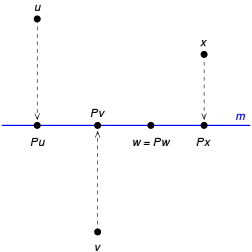
\includegraphics[scale=0.5]{projection.png}\\

\underline{\textit{Process}}\\
Let $W \subset \real^n$ be a plane and $v \in \real^{n+1}$ be a point.
\begin{enumerate}[label=\roman*)]
  \itemsep0em
  \item Find an orthonormal basis for $W$, $\{x_1, \dots, x_n\}$;
  \item Define the projection $P(v) = \innerproduct{x_1}{v}x_1 + \dots + \innerproduct{x_n}{v}x_n$;
  \item Then $P(v)$ is the vector from $v$ to the closest point on $W$;
  \item So $\|P(v)\|$ is the distance of $v$ from $W$.
\end{enumerate}

\underline{\textit{Example}}\\
Let $W = span\left(\left\{(1, 1, 1, 1), (-1, 4, 4, 1), (4, -2, 2, 0)\right\}\right) \subset \real^4$.
Find the distance of $\vect{v} = (1,2,3,4)$ from $W$.\\

$W$ has an orthonormal basis of $\begin{pmatrix} 1/2 \\ 1/2 \\ 1/2 \\ 1/2 \end{pmatrix}, \begin{pmatrix} -1/\sqrt{2} \\ \sqrt{2}/3 \\ \sqrt{2}/3 \\ -1/3\sqrt{2} \end{pmatrix}\ \&\ \begin{pmatrix} 1/2\sqrt{3} \\ -5/6\sqrt{3} \\ 7/6\sqrt{3} \\ -5/6\sqrt{3} \end{pmatrix}$.\\
Then\\
\[\begin{array}{rcccl}
  \innerproduct{\vect{x}_1}{\vect{v}} &=& \frac{1}{2}(1 + 2 + 3 + 4) &=& 5\\
  \innerproduct{\vect{x}_2}{\vect{v}} &=& \frac{1}{3\sqrt{2}}(-3+4+6-4) &=& \frac{1}{\sqrt{2}}\\
  \innerproduct{\vect{x}_3}{\vect{v}} &=& \frac{1}{2\sqrt{3}}(1 + \frac{10}{3} + 7 - \frac{20}{3}) &=& \frac{-1}{\sqrt{3}}
\end{array}\]
So $\displaystyle{P(\vect{v}) = 5\vect{x}_1 + \frac{1}{\sqrt{2}}\vect{x}_2 - \frac{1}{\sqrt{3}}\vect{x}_3 = \left(\frac{11}{6}, \frac{28}{9}, \frac{22}{9}, \frac{47}{18}\right)}$\\
$\displaystyle{\left\|\vect{v} - P(\vect{v})\right\| = \left\|\left(\frac{-5}{6}, \frac{-10}{9}, \frac{5}{9}, \frac{25}{18} \right)\right\| = \underline{\frac{5}{\sqrt{6}}}}$\\

\textbf{Hermitian}\\

\underline{\textit{Theory}}\\
A square matrix, $A \in M_n(\field)$, is a \textit{hermitian} if $A = \bar{A^t} = A^*$.\\
\underline{i.e.} $A$ equals the complex conjugate of its transpose.\\
The eigenvectors of a hermitian form an orthonormal basis.\\
$A$ is \textit{unitary} if $AA^* = I$.\\

\underline{\textit{Adjoint Operator}}\\
Let $T$ be a linear operator.\\
The adjoint operator, $T^*$, of $T$ is defined such that $\innerproduct{v}{T(w)} = \innerproduct{T^*{v}}{w}$.\\
This maintains the properties of the inner product.\\

\underline{\textit{Normal Matrix}}\\
A matrix, $A$, is normal if $AA^* = A^*A$.\\
This means $A^* = A^t$ or $A^* = A^{-1}$.

\end{document}
